\documentclass[12pt]{report}

\title{A Mathematics Student's Lament}

\usepackage{authblk}

\author[1]{Nicholas Arvanitellis}
\author[2]{\\Jacob Bos}
\author[3]{\\Marcel Reverter-Rambaldi}

\affil[1,2,3]{Australian National University}
\affil[3]{The University of Queensland}



\usepackage{graphicx}
\usepackage{amsmath}
\usepackage{amssymb}
\usepackage{amsfonts}
\usepackage{amsthm}

\usepackage{float}

\usepackage{multicol}
\setlength{\columnsep}{1cm}

%\usepackage{setspace}

\usepackage[margin=2cm]{geometry}

\usepackage{xcolor}

\usepackage{titlesec}

\titleformat{\section}
{\color{purple}\normalfont\Large\bfseries}
{\color{purple}\thesection}{1em}{}

\titleformat{\subsection}
{\color{purple}\normalfont\bfseries}
{\color{purple}\thesubsection}{1em}{}

\titleformat{\subsubsection}
{\color{blue}\normalfont\bfseries}
{\color{blue}\thesubsubsection}{1em}{}


\begin{document}

    \maketitle
    \tableofcontents
\newpage


% ================================================================================================
% === Intro              =========================================================================
% ================================================================================================
\chapter{Introduction}




% ================================================================================================
% === Ch2 - The HSC ==============================================================================
% ================================================================================================
\chapter{The HSC}




% ================================================================================================
% === Ch3 - The SACE =============================================================================
% ================================================================================================
\chapter{The SACE}

\section{Stage 1}
\subsection{Essential Mathematics}

    According to the SACE subject outline, Stage 1 Essential Mathematics covers the following topics.
    \begin{table}[H]
        \centering
        \begin{tabular}{|l|l|}
        \hline
            1 & Calculations, time, and ratio \\ \hline
            2 & Earning and spending \\ \hline
            3 & Geometry \\ \hline
            4 & Data in context \\ \hline
            5 & Measurement \\ \hline
            6 & Investing \\ \hline
            7 & Open topic \\ \hline
        \end{tabular}
    \end{table}

\subsection{General Mathematics}

    According to the SACE subject outline, Stage 1 General Mathematics covers the following topics.
    \begin{table}[H]
        \centering
        \begin{tabular}{|l|l|}
        \hline
            1 & Investing and borrowing \\ \hline
            2 & Measurement \\ \hline
            3 & Statistical investigation \\ \hline
            4 & Applications of trigonometry \\ \hline
            5 & Linear and exponential functions and their graphs \\ \hline
            6 & Matrices and networks \\ \hline
            7 & Open topic \\ \hline
        \end{tabular}
    \end{table}

\subsection{Mathematics}

    According to the SACE subject outline, Stage 1 Mathematics covers the following topics.
    \begin{table}[H]
        \centering
        \begin{tabular}{|l|l|}
        \hline
            1 & Functions and Graphs \\ \hline
            2 & Polynomials \\ \hline
            3 & Trigonometry \\ \hline
            4 & Counting and Statistics \\ \hline
            5 & Growth and Decay \\ \hline
            6 & Introduction to Differential Calculus \\ \hline
            7 & Arithmetic and geometric series and sequences \\ \hline
            8 & Geometry \\ \hline
            9 & Vectors in the plane \\ \hline
            10 & Further Trigonometry \\ \hline
        \end{tabular}
    \end{table}


% ///////////////////////////////////////////////////////////////////////////////////////////////////
\section{Stage 2}
\subsection{Essential Mathematics}

    According to the SACE subject outline, Stage 2 Essential Mathematics covers the following topics.
    \begin{table}[H]
        \centering
        \begin{tabular}{|l|l|}
        \hline
            1 & Scales, plans, and models \\ \hline
            2 & Measurement \\ \hline
            3 & Business applications \\ \hline
            4 & Statistics \\ \hline
            5 & Investments and loans \\ \hline
            6 & Open topic \\ \hline
        \end{tabular}
    \end{table}

\subsection{General Mathematics}

    According to the SACE subject outline, Stage 2 General Mathematics covers the following topics.
    \begin{table}[H]
        \centering
        \begin{tabular}{|l|l|}
        \hline
            1 & Modelling with linear relationships \\ \hline
            2 & Modelling with matrices \\ \hline
            3 & Statistical models \\ \hline
            4 & Financial models \\ \hline
            5 & Discrete models \\ \hline
            6 & Open topic \\ \hline
        \end{tabular}
    \end{table}


\subsection{Mathematical Methods}

    According to the SACE subject outline, Stage 2 Mathematical Methods covers the following topics.
    \begin{table}[H]
        \centering
        \begin{tabular}{|l|l|}
        \hline
            1 & Further differentiation and applications \\ \hline
            2 & Discrete random variables \\ \hline
            3 & Integral calculus \\ \hline
            4 & Logarithmic functions \\ \hline
            5 & Continuous random variables \\ \hline
            6 & Sampling and confidence intervals \\ \hline
        \end{tabular}
    \end{table}

\subsection{Specialist Mathematics}

    According to the SACE subject outline, Stage 2 Mathematical Methods covers the following topics.
    \begin{table}[H]
        \centering
        \begin{tabular}{|l|l|}
        \hline
            1 & Mathematical induction \\ \hline
            2 & Complex numbers \\ \hline
            3 & Functions and sketching graphs \\ \hline
            4 & Vectors in three dimensions \\ \hline
            5 & Integration techniques and applications \\ \hline
            6 & Rates of change and differential equations \\ \hline
        \end{tabular}
    \end{table}

% ================================================================================================
% === Ch4 - The QCE =============================================================================
% ================================================================================================
\chapter{The QCE}





% ================================================================================================
% === ChX - What's Missing? ======================================================================
% ================================================================================================
\chapter{What's Missing?}




% ================================================================================================
% === ChY.1 - Stage 1 ============================================================================
% ================================================================================================
\chapter{An Alternative}

\begin{figure}[H]
    \centering
    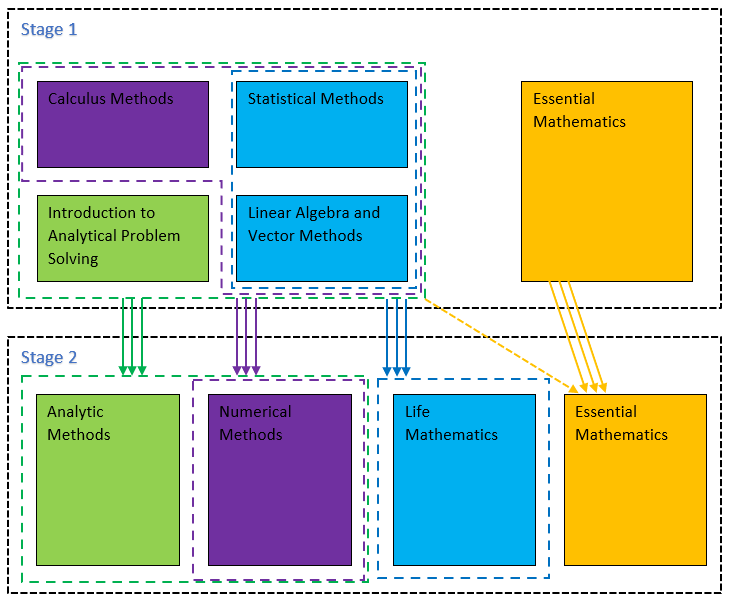
\includegraphics[width=0.8\textwidth]{Flowchart1.jpg}
    \caption{Subject structure}
\end{figure}

\section{Stage 1 - Year 11}

    \begin{table}[H]
        \centering
        \begin{tabular}{|l|l|}
        \hline
            S1.1 & The notion of probability and nPr/nCr Calculations \\ \hline
            S1.2 & Measures and Centre and Spread \\ \hline
            S2 & Continuous random variables \\ \hline
            S3 & Sampling, confidence intervals and hypothesis testing\\ \hline \hline \hline

            L1 & Geometric Trigonometry \\ \hline
            L2 & Vectors in the plane \\ \hline
            L3 & Matrices, networks and linear systems\\ \hline \hline \hline

            C1.1 & Functions and Graphs \\ \hline
            C1.2 & Polynomials \\ \hline
            C2.1 & Trigonometric functions \\ \hline
            C2.2 & Growth and Decay \\ \hline
            C3 & Introduction to Differential Calculus \\ \hline \hline \hline

            A1 & Geometry, Mathematical Problem Solving and Direct Proofs\\ \hline
            A2 & Sets, Elementary Set Operations and Relations\\ \hline
            A3 & Sequences, Series and Inductive Proofs\\ \hline
            AX & The map of mathematics\\ \hline
        \end{tabular}\\
        \caption{Main Cluster}
    \end{table}

\subsection{Essential Mathematics}
\subsection{Statistical Methods}
\subsection{Calculus Methods}
\subsection{Linear Algebra Methods}
\subsection{Introduction to Analytical Problem Solving}

% ================================================================================================
% === ChY.2 - Stage 2 ============================================================================
% ================================================================================================
\section{Stage 2 - Year 12}

\subsection{Essential Mathematics}
\subsection{Life Mathematics}
\subsection{Analytical Methods}
    Analytical methods should serves to develop the analytical skills necessary for the mathematical, engineering and physical sciences and an appreciation of proof, logic and the fundamental structures of mathematics.

    Proposed topics are:
    \begin{table}[H]
        \centering
        \begin{tabular}{|l|l|}
        \hline
            1.1 & Logic and Proofs \\ \hline
            1.2 & Introduction to algebra and real analysis \\ \hline
            2 & Functions and graphs \\ \hline 
            3 & Polynomials and Complex numbers \\ \hline
            4 & Analytic Integration  \\ \hline 
            5.1 & Analytic solutions to differential equations \\ \hline
            5.2 & Vectors and Vector Calculus in three dimensions\\ \hline
        \end{tabular}
    \end{table}

    \subsubsection{Introduction to mathematics}
        \paragraph*{Logic and Proofs} Students should become familiar with logical notation such as $\forall$, $\exists$, $\and$ and the negation of simple statements. This should lead to discussions of contrapositive and contradiction based proofs. Direct and Inductive proofs should be revised and truth tables explored.

        \paragraph*{Introduction to algebra and real analysis} Introduce real analysis and discuss the logic for $\varepsilon - N$ and $\varepsilon - \delta$ limit definitions. The notion of a group should be introduced with discussion of permutation groups and cyclic groups. Discuss how such structures underly almost all mathematics.

    \subsubsection{Functions and Graphs} Discuss the definition of a graph and what fulfils this definition. Study features of graphs of rational functions including roots, poles and asymptotes including applying $\varepsilon-\delta$ proofs. Introduce polynomial division and polynomial long division.

    \subsubsection{Polynomials and Complex Numbers} Introduce and prove the factor and remainder theorems and apply the fundamental theorem of calculus. Demonstrate how finding the solutions to polynomials led to the invention of complex numbers discuss and prove complex conjugate root theorem. Discover the nth roots of unity and their realization as a cyclic group.

    \subsubsection{Analytic integration} Introduce and prove the integration by parts formula and how to apply it including the LIATE acronym. Introduce the derivatives of $\arccos$, $\arcsin$ and $arctan$ in the context of integration by substitution. Apply trigonometric identities to the integration of functions such as $\cos^2x$, $\cos^3x$ and $\tan^2x$. Discuss volumes of revolution around $x$ and $y$ axes.


    \subsubsection{Differential equations, vectors and vector calculus}
        \paragraph*{Analytic solutions to differential equations} Discuss implicit differentiation and separable differential equations. Be able to solve simple separable equations such as the harmonic oscillator and logistic growth. Small discussion of related rates.
        
        \paragraph*{Vectors and Vector Calculus in three dimensions} Discuss scalar fields in 2d and 3d and partial differentiation. Link parametric equations to related rates.



\subsection{Numerical Methods}
    
    Skills in numerical modelling and computation are incredibly important to all sciences with the authours having expressed  how important such skills are in preparing for university studies in multiple disciplines. Numerical Methods aims to address this shortcoming by developing the topics learned in stag 1 with emphasis computing. Students will be left with the appreciation of computer driven calculation necessary for further study in engineering, the sciences and economics.


    The language Julia has been recommended by the authours due to it having syntax familiar to users of both MATLAB and Python but with the capabilities of MATLAB and R (commonly used in university) inbuilt requiring no imported LA or Statistical packages to achieve the aims of the course. This eases the barrier of entry to students whilst also being free (including when pared with an IDE like VS Code).

    Proposed topics are:
    \begin{table}[H]
        \centering
        \begin{tabular}{|l|l|}
        \hline
            1.1 & Introduction to computational approaches and the julia language\\ \hline
            1.2 & Revision of common differential functions\\ \hline
            2 & Further differentiation and applications \\ \hline
            3 & Integral calculus \\ \hline
            4 & Discretization of calculus models\\ \hline
            5 & Computational linear algebra \\ \hline
            6.1 & Statistics and computation \\ \hline
            6.2 & Computational problem solving \\ \hline
        \end{tabular}
    \end{table}

    \subsubsection{Introduction and revision} As commonly done students should first revise logarithmic, exponential and trigonometric functions for later use in calculus. Subsequently the Julia language should be introduced and the motivation behind the choice. Students should then have a practical understanding variables, simple types, digital boolean logic including \verb|If-Then-Else| statements and loops such as \verb|for|, \verb|while| and recursion. Students should understand the difference between scripting and repl based interaction.
    
    \subsubsection{Further differentiation and applications} Students should be able to differentiate trigonometric, exponential and logarithmic functions. They should also understand the chain product and quotient rules.

    \subsubsection{Integral calculus} Understand antidifferentiation, the fundamental theorem of calculus and integrating trigonometric and exponential functions.

    \subsubsection{Discretization of calculus models} Cover the discretization of calculus problems and implement in Julia discrete differentiation, the midpoint rule, trapezoid rule and simpson's rule. Introduce differential equations and how to simulate their behaviour such as harmonic oscillators. Understand the precision of their algorithms.

    \subsubsection{Computational linear algebra} Be able to perform elementary row operations to reduced row echelon form and solve consistent systems of linear equations. Understand geometrical interpretation of inconsistent systems in $\mathbb{R}^2$ and $\mathbb{R}^3$. Write both row reduction Cramer's rule algorithms so find solutions to consistent systems. Find the shortest distance between planes and line problems in n dimensions. Be able to simulate markov chains and compute steady states as well as matrix transformations.

    \subsubsection{Further computation} 
        \paragraph*{Statistics and computation} Import .csv files and navigate datasets using julia. Perform visualization and statistical analysis on large datasets applying previously learned statistics.

        \paragraph*{Computational problem solving} Study intersectional areas such as Monte-carlo methods, financial applications, and reason on algorithmic complexity (linear, quadratic and exponential time). Select topics from cellular automata and introduce simple game strategies in theory such as greedy and minimax. Present a map of numerical and computational fields.

\end{document}